\documentclass[review,
3p]{elsarticle} %review=doublespace preprint=single 5p=2 column
%%% Begin My package additions %%%%%%%%%%%%%%%%%%%

\usepackage[hyphens]{url}

  \journal{Malaria Journal} % Sets Journal name

\usepackage{lineno} % add

\usepackage{graphicx}
%%%%%%%%%%%%%%%% end my additions to header

\usepackage[T1]{fontenc}
\usepackage{lmodern}
\usepackage{amssymb,amsmath}
\usepackage{ifxetex,ifluatex}
\usepackage{fixltx2e} % provides \textsubscript
% use upquote if available, for straight quotes in verbatim environments
\IfFileExists{upquote.sty}{\usepackage{upquote}}{}
\ifnum 0\ifxetex 1\fi\ifluatex 1\fi=0 % if pdftex
  \usepackage[utf8]{inputenc}
\else % if luatex or xelatex
  \usepackage{fontspec}
  \ifxetex
    \usepackage{xltxtra,xunicode}
  \fi
  \defaultfontfeatures{Mapping=tex-text,Scale=MatchLowercase}
  \newcommand{\euro}{€}
\fi
% use microtype if available
\IfFileExists{microtype.sty}{\usepackage{microtype}}{}
\usepackage[]{natbib}
\bibliographystyle{model6-num-names}

\ifxetex
  \usepackage[setpagesize=false, % page size defined by xetex
              unicode=false, % unicode breaks when used with xetex
              xetex]{hyperref}
\else
  \usepackage[unicode=true]{hyperref}
\fi
\hypersetup{breaklinks=true,
            bookmarks=true,
            pdfauthor={},
            pdftitle={How many nets are needed to reach universal coverage - an update},
            colorlinks=false,
            urlcolor=blue,
            linkcolor=magenta,
            pdfborder={0 0 0}}

\setcounter{secnumdepth}{0}
% Pandoc toggle for numbering sections (defaults to be off)
\setcounter{secnumdepth}{0}


% tightlist command for lists without linebreak
\providecommand{\tightlist}{%
  \setlength{\itemsep}{0pt}\setlength{\parskip}{0pt}}

% From pandoc table feature
\usepackage{longtable,booktabs,array}
\usepackage{calc} % for calculating minipage widths
% Correct order of tables after \paragraph or \subparagraph
\usepackage{etoolbox}
\makeatletter
\patchcmd\longtable{\par}{\if@noskipsec\mbox{}\fi\par}{}{}
\makeatother
% Allow footnotes in longtable head/foot
\IfFileExists{footnotehyper.sty}{\usepackage{footnotehyper}}{\usepackage{footnote}}
\makesavenoteenv{longtable}


\usepackage{floatrow}
\floatsetup[figure]{capposition=top}
\floatplacement{figure}{H}
\usepackage{setspace}\doublespacing
\biboptions{sort&compress}
\usepackage{booktabs}
\usepackage{longtable}
\usepackage{array}
\usepackage{multirow}
\usepackage{wrapfig}
\usepackage{float}
\usepackage{colortbl}
\usepackage{pdflscape}
\usepackage{tabu}
\usepackage{threeparttable}
\usepackage{threeparttablex}
\usepackage[normalem]{ulem}
\usepackage{makecell}
\usepackage{xcolor}
\usepackage{amsmath}
\usepackage{caption}



\begin{document}


\begin{frontmatter}

  \title{How many nets are needed to reach universal coverage - an
update}
    \author[Tropical Health LLP]{Hannah Koenker}
   \ead{hannah@trophealth.com} 
    \author[International Federation of the Red Cross and Red Crescent
Societies]{Marcy Erskine}
   \ead{marcy.erskine@ifrc.org} 
    \author[International Federation of the Red Cross and Red Crescent
Societies]{Robert Opoku}
   \ead{robert.opoku@ifrc.org} 
    \author[Tropical Health LLP]{Eleanore Sternberg}
   \ead{eleanore@trophealth.com} 
      \affiliation[Tropical Health LLP]{Baltimore, USA}
    \cortext[cor1]{Corresponding author}
  
  \begin{abstract}
  {[}350 words max{]}
  \end{abstract}
    \begin{keyword}
    insecticide-treated nets \sep 
    long-lasting insecticidal nets
  \end{keyword}
  
 \end{frontmatter}

\hypertarget{background}{%
\section{Background}\label{background}}

Insecticide treated nets (ITNs) have served as the cornerstone of
malaria vector control in sub-Saharan Africa for the past two decades.
Over 2.5 billion ITNs have been delivered to countries
\citep{Milliner:2016um}, primarily through periodic mass distribution
campaigns scheduled at approximately three-year intervals, aligning with
the expected lifespan of nets. Recent work has shown significant
variation in ITN durability across geographic zones, and while some
studies support a three-year median lifespan, multi-country analyses of
ITN retention times indicate half of countries can expect two years or
less of useful life for the majority of nets they distribute
\citep{10.1038/s41467-021-23707-7}. The implications of
shorter-than-expected retention times have important implications for
the way countries quantify ITN commodity need for mass campaigns, and
raise several key questions. First, what is the projected impact of the
mismatch in campaign cycle and ITN retention in terms of overall ITN
coverage? Second, if mass campaigns every three years are insufficient
due to ITNs lasting only 1-2 years, is switching to a two-year campaign
cycle indicated, or are there alternative or supplemental ways to
distribute ITNs to ensure high rates of ITN access are maintained over
time? Third, with what we know now about ITN retention and ITN
distribution modalities, is population divided by 1.8 (as currently
recommended \citep{WorldHealthOrganization:2019ws}) the correct
quantification approach for mass campaigns for all countries? Finally,
what would optimum ITN quantification look like for countries given
their particular ITN retention times, aiming to sustain high levels of
ITN access (the necessary, but not sufficient, precursor to ITN use)?

This paper explores these questions using an existing stock and flow
model \citep{10.1186/s12936-022-04272-w} to project population ITN
access for countries in sub-Saharan Africa over five different
distribution scenarios, using estimated ITN retention times from
Bertozzi-Villa et al \citep{10.1038/s41467-021-23707-7} and varying
quantification approaches within each distribution scenario.

\hypertarget{methods}{%
\section{Methods}\label{methods}}

\hypertarget{projections-of-future-coverage}{%
\subsection{Projections of future
coverage}\label{projections-of-future-coverage}}

Each country was assigned an indicative population of 10 million people
in the database, starting in 2020, and an annual population growth rate
of 3\%, as the model outputs are adjusted for population and thus do not
require specific population estimates.

ITNs were distributed in the model for each scenario as shown in Table
1.

\begin{longtable}[]{@{}
  >{\raggedright\arraybackslash}p{(\columnwidth - 6\tabcolsep) * \real{0.1391}}
  >{\raggedright\arraybackslash}p{(\columnwidth - 6\tabcolsep) * \real{0.3435}}
  >{\raggedright\arraybackslash}p{(\columnwidth - 6\tabcolsep) * \real{0.2087}}
  >{\raggedright\arraybackslash}p{(\columnwidth - 6\tabcolsep) * \real{0.3087}}@{}}
\caption{Distribution Scenarios and their ITN inputs}\tabularnewline
\toprule
\begin{minipage}[b]{\linewidth}\raggedright
Scenario
\end{minipage} & \begin{minipage}[b]{\linewidth}\raggedright
Mass Campaign
\end{minipage} & \begin{minipage}[b]{\linewidth}\raggedright
ANC/EPI (routine)
\end{minipage} & \begin{minipage}[b]{\linewidth}\raggedright
Annual school/ community
\end{minipage} \\
\midrule
\endfirsthead
\toprule
\begin{minipage}[b]{\linewidth}\raggedright
Scenario
\end{minipage} & \begin{minipage}[b]{\linewidth}\raggedright
Mass Campaign
\end{minipage} & \begin{minipage}[b]{\linewidth}\raggedright
ANC/EPI (routine)
\end{minipage} & \begin{minipage}[b]{\linewidth}\raggedright
Annual school/ community
\end{minipage} \\
\midrule
\endhead
1. ``Status Quo'' & In 2022, 2025, 2028, 2031, 2034 at population / 1.8
& 2020-2035, varying from 5-7\% of the population & none \\
2. ``Full-scale continuous'' & In 2020, to establish high coverage at
population / 1.8 & 2021-2035 at 6\% of the population & 2022-2032
varying from 1-20\% of the population \\
3. ``Mass plus continuous'' & In 2022, 2025, 2028, 2031, 2034 at
population / 1.8 & 2020-2035 at 6\% of the population & Only in years
between campaigns, varying from 1-20\% of the population \\
4. ``Varying 3-year mass'' & In 2022, 2025, 2028, 2031, 2034, varying
from population / 1.0-2.0 & 2020-2035 at 6\% of the population & none \\
5. ``Varying 2-year mass'' & In 2022, 2024, 2026, 2028, 2030, 2032, 2034
varying from population / 1.0-2.0 & 2020-2035 at 6\% of the population &
none \\
\bottomrule
\end{longtable}

For each year, the stock and flow model used a country-specific
estimated median lifespan from Bertozzi-Villa et al
\citep{10.1038/s41467-021-23707-7} to decay each crop of distributed
nets annually. The net decay functions rely on smooth-compact loss
function developed by Nakul Chitnis and described in Koenker et al and
Bhatt et al
\citep{Koenker:2013ed, Bhatt:2015gn, 10.1186/s12936-022-04272-w}, and
are shown in Fig. \ref{ret_decay_fig}.

\begin{verbatim}
## pdf 
##   2
\end{verbatim}

\begin{figure}
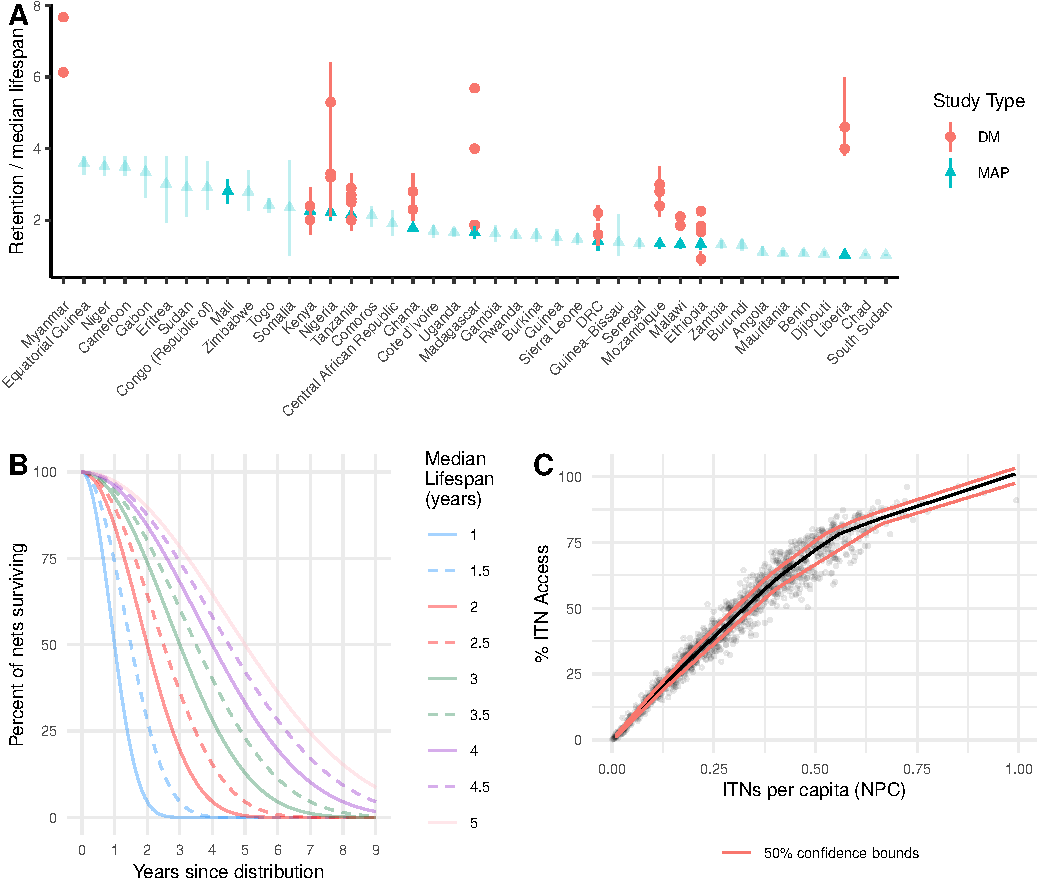
\includegraphics[width=0.8\linewidth]{quant_paper_files/figure-latex/ret_decay_fig-1} \caption{\label{ret_decay_fig}A) ITN retention times and median lifespans estimated from durability monitoring studies B) Smooth-compact loss function for net decay C) nonparametric conditional quartile function for ITN access as a function of NPC}\label{fig:ret_decay_fig}
\end{figure}

The total net crop (consisting of all surviving nets from various
channels to date) was summed for each year and country. This was then
divided by the population projected to calculate nets-per-capita (NPC)
in each year and council.

To estimate ITN access from NPC, a nonparametric conditional quartile
function for ITN access as a function of NPC was estimated from 124
demographic health survey data and malaria indicator surveys (MIS). A
grid of 100 points was produced and used to predict ITN access from NPC
(Fig. \ref{ret_decay_fig}). Confidence intervals for both estimated
median lifespan and the function of ITN access vs NPC were used to
generate an overall confidence interval around the estimate of ITN
access.

To further understand the relative sizes of ITN distributions through
various channels, total ITNs delivered per channel were divided by the
population and expressed as ``nets issued as a percentage of the
population'' (NPP).

\hypertarget{scenarios}{%
\subsection{Scenarios}\label{scenarios}}

To inform recommendations for quantification of ITNs, the above process
was used to model ITN distributions under five typical ITN distribution
scenarios, varying quantification approaches within each scenario. The
majority of malaria-endemic countries currently implement Scenario 1;
Tanzania is an example of Scenario 2, while Ghana exemplifies Scenario
3. While countries aim to deliver mass campaigns every three years, some
have recently argued for campaign every two years to offset shorter
median net lifespans.

\begin{enumerate}
\def\labelenumi{\arabic{enumi}.}
\tightlist
\item
  ``Status Quo'': Mass campaigns every three years with routine
  distribution of ITNs to pregnant women and infants through antenatal
  clinics (ANC) and immunization visits (EPI). Quantification of the
  mass campaigns was fixed at population / 1.8 while quantification of
  routine distribution varied from population x 5\%-7\%.
\item
  ``Full-scale continuous'': Full-scale annual school distribution of
  ITNs with routine distribution of ANC and EPI ITNs, fixing the routine
  distribution at population x 6\% and varying the quantification of
  school distributions from population x 1-20\%
\item
  ``Mass plus continuous'': Mass campaign every three years with routine
  distribution of ANC and EPI ITNs and with annual school distribution
  in a limited number of classes, or limited community distribution in
  the years between campaigns. Quantification of the mass campaigns was
  fixed at population / 1.8 and routine distribution at population x
  6\%, varying the annual school/community distribution between
  population x 7-25\%.
\item
  ``Varying 3-year mass'': Mass campaigns every three years with routine
  distribution of ITNs to pregnant women and infants through antenatal
  clinics (ANC) and immunization visits (EPI). Quantification of routine
  distribution was fixed at 6\%, and quantification of the mass
  campaigns was varied from population / 1.0 to population / 2.0 in
  increments of 0.1.
\item
  ``Varying 2-year mass'': Mass campaigns every two years with routine
  distribution of ITNs to pregnant women and infants through antenatal
  clinics (ANC) and immunization visits (EPI). Quantification of routine
  distribution was fixed at 6\%, and quantification of the mass
  campaigns was varied from population / 1.0 to population / 2.0 in
  increments of 0.1.
\end{enumerate}

All scenarios with mass campaigns began with a mass campaign in 2022 and
ended in 2035. The ``full scale continuous'' scenario assumed a mass
campaign (quantified with population / 1.8) in 2020 to scale up coverage
prior to switching over to a fully continuous ITN strategy.

To assess feasibility of large-scale school distribution in relation to
optimal quantification factors, the proportion of the population that
are primary school students currently attending school was calculated
from the most recent Demographic and Health Surveys for each country,
obtained with permission from dhsprogram.com.

\hypertarget{results}{%
\section{Results}\label{results}}

Given a target of 80\% ITN access, the recommended quantification
approaches for each scenario varied considerably across countries,
driven primarily by the median retention time. Recommended
quantification approaches are summarized for the scenarios that include
continuous distribution in Table 2, for 3-year mass campaigns in Table
3, and for 2-year mass campaigns in Table 4.

For Scenario 2, which relies on full-scale annual continuous
distribution in combination with routine ANC/EPI ITN delivery to
maintain access, the annual quantifier needed to maintain ITN access at
70\% ranged from 7\% of the population in Cameroon and The Gambia, to
26\% of the population in Benin, Djibouti, Liberia, Mauritania, South
Sudan, and Chad. Similarly, to maintain ITN access at 80\%, the
quantifier ranged from 10\% for Cameroon and Gabon, to 30\% for Angola.
In only a few countries was ITN access able to reach 90\% - from 17\% of
the population in Cameroon, to 30\% in Angola, Cote d'Ivoire,
Madagascar, and Uganda.

For Scenario 3, where mass campaigns are conducted every three years,
routine ITNs through ANC/EPI are conducted consistently, and continuous
distribution supplements ITN access in the years between campaigns,
there was also a range of quantifiers for the annual continuous
distribution channels. At the 70\% target, many countries required ITNs
equivalent to 7\% of the population, but this rose to 25\% for Liberia,
South Sudan, and Chad. At the 80\% target, some countries still achieved
this with 7\% of the population in ITNs between campaigns, while Benin
and Mauritania are estimated to need 30\% of the population in ITNs.
Several countries were able to maintain ITN access at 90\% with only
limited inputs from the continuous channel, at 7\% of the population,
including Cameroon, Mali, Niger, and Zimbabwe.

\captionsetup[table]{labelformat=empty,skip=1pt}
\begin{longtable}{lrrrrrr}
\caption*{
{\large Minimum quantifier to sustain ITN access at target level}
} \\ 
\toprule
 & \multicolumn{3}{c}{Scenario 2 (full continuous strategy)} & \multicolumn{3}{c}{Scenario 3 (continuous between mass campaigns)} \\ 
\cmidrule(lr){2-4} \cmidrule(lr){5-7}
 & \multicolumn{6}{c}{Targeted ITN access} \\ 
\cmidrule(lr){2-7}
Country Code & 70\% & 80\% & 90\% & 70\% & 80\% & 90\% \\ 
\midrule
AO & 25 & 30 &  & 23 & 29 &  \\ 
BF & 19 & 25 &  & 11 & 17 & 28 \\ 
BI & 23 & 29 &  & 17 & 23 & 26 \\ 
BJ & 26 &  &  & 23 & 30 &  \\ 
CD & 22 & 28 &  & 15 & 21 & 28 \\ 
CF & 15 & 24 & 28 & 7 & 10 & 22 \\ 
CG & 9 & 12 & 20 & 7 & 7 & 11 \\ 
CI & 19 & 29 & 30 & 9 & 14 & 26 \\ 
CM & 7 & 10 & 17 & 7 & 7 & 7 \\ 
DJ & 26 &  &  & 24 & 21 &  \\ 
ER & 9 & 12 & 20 & 7 & 7 & 10 \\ 
ET & 23 & 29 &  & 17 & 23 & 30 \\ 
GA & 7 & 10 & 17 & 7 & 7 & 8 \\ 
GH & 17 & 27 & 29 & 8 & 7 & 24 \\ 
GM & 21 & 25 &  & 11 & 16 & 27 \\ 
GN & 20 & 26 &  & 13 & 19 & 30 \\ 
GQ & 7 & 10 & 16 & 7 &  & 7 \\ 
GW & 22 & 28 &  & 16 & 22 & 29 \\ 
KE & 12 & 17 & 27 & 7 & 7 & 15 \\ 
KM & 13 & 19 & 28 & 7 & 8 & 16 \\ 
LR & 26 &  &  & 25 & 22 &  \\ 
MG & 20 & 24 & 30 & 10 & 15 & 27 \\ 
ML & 9 & 12 & 21 & 7 & 7 & 7 \\ 
MR & 26 &  &  & 23 & 30 &  \\ 
MW & 23 & 29 &  & 17 & 23 & 30 \\ 
MZ & 22 & 28 &  & 17 & 23 & 30 \\ 
NE & 7 & 10 & 17 & 7 & 7 & 7 \\ 
NG & 12 & 18 & 27 & 7 & 7 & 15 \\ 
RW & 21 & 25 &  & 11 & 17 & 28 \\ 
SD & 9 & 12 & 20 & 7 & 7 & 11 \\ 
SL & 21 & 27 &  & 14 & 20 & 30 \\ 
SN & 22 & 28 &  & 16 & 22 & 30 \\ 
SO & 12 & 16 & 26 & 7 & 7 & 14 \\ 
SS & 27 &  &  & 25 & 22 &  \\ 
TD & 26 &  &  & 25 & 22 &  \\ 
TG & 11 & 15 & 25 & 7 & 7 & 13 \\ 
TZ & 13 & 19 & 28 & 7 & 8 & 16 \\ 
UG & 20 & 24 & 30 & 10 & 15 & 26 \\ 
ZM & 23 & 29 &  & 17 & 23 & 30 \\ 
ZW & 9 & 12 & 21 & 7 & 7 & 7 \\ 
\bottomrule
\end{longtable}

For Scenario 4, the quantifier used for 3-year mass campaigns (in
combination with routine ITN distribution at ANC/EPI clinics) was varied
from 1.0 to 2.0. The lowest level of ITN access between campaigns is
shown in Table 3. Under the current recommended quantifier of 1.8, only
Cameroon, Eritrea, Gabon, and Niger were estimated to maintain ITN
access at or above 80\% between campaigns.

Table 4 provides a similar picture but for campaigns conducted every 2
years. Under a population / 1.8 quantifier, CAR, Congo, Cote d'Ivoire,
Cameroon, Eritrea, Gabon, Ghana, the Gambia, Kenya, Madagascar, Mali,
Niger, Nigeria, Sudan, Togo, Tanzania, Uganda, and Zimbabwe would all
maintain ITN access at or above 80\% between campaigns. In other
countries, 2-yearly campaigns closer to one ITN per person in order to
maintain ITN access at the 80\% target.

Figures 2-4 illustrate scenario results for each country, for scenarios
1 (Figure 2), scenario 2 (Figure 3), and scenario 3 (Figure 4). Inputs
of ITNs are indicated in orange for each year; the resulting population
ITN access estimate is shown in green. The typical rise and fall of ITN
access is apparent in Figures 2 and 4, while ITN access is maintained at
a steady rate in Figure 3 where distributions are annual through
continuous channels.

test stuff

more test stuff

\textbackslash begin\{figure\}
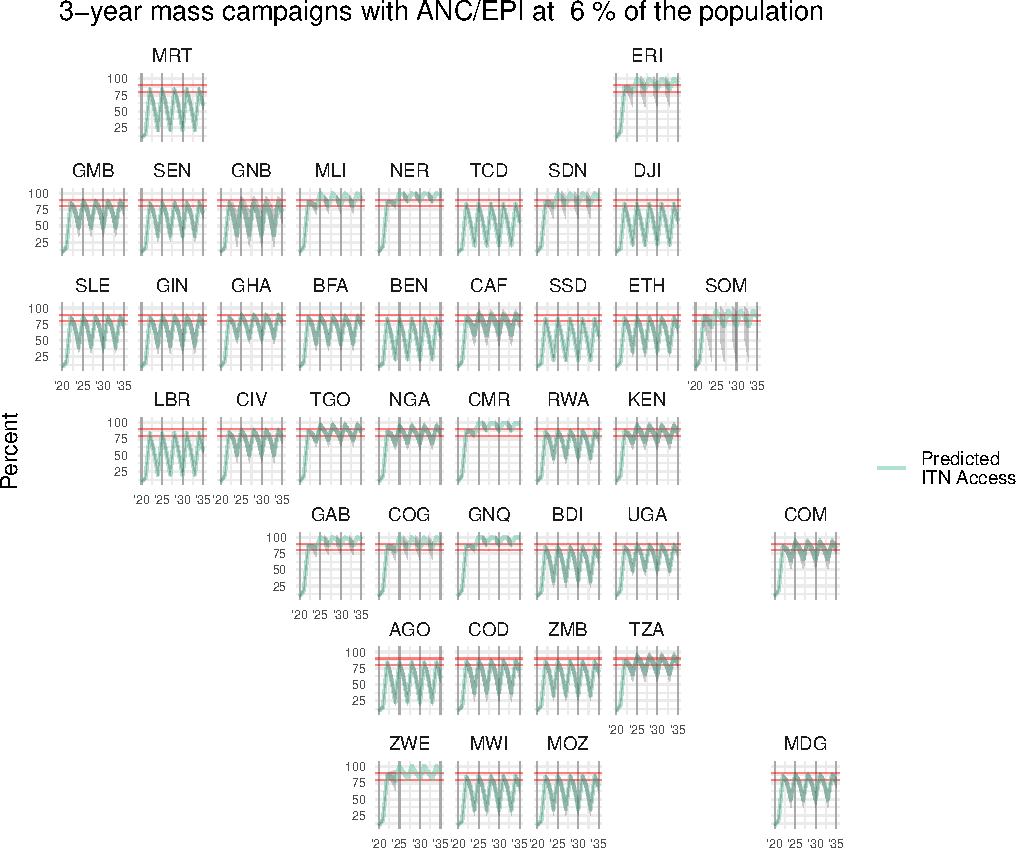
\includegraphics[width=0.8\linewidth]{quant_paper_files/figure-latex/geo_facets_3ucc-1}
\textbackslash caption\{\label{geo_facets_3ucc}ITN access estimated for
3-year mass campaign strategy, with ANC/EPI distribution at 6\% of the
population annually\}\label{fig:geo_facets_3ucc}
\textbackslash end\{figure\}

additional test stuff

\textbackslash begin\{figure\}
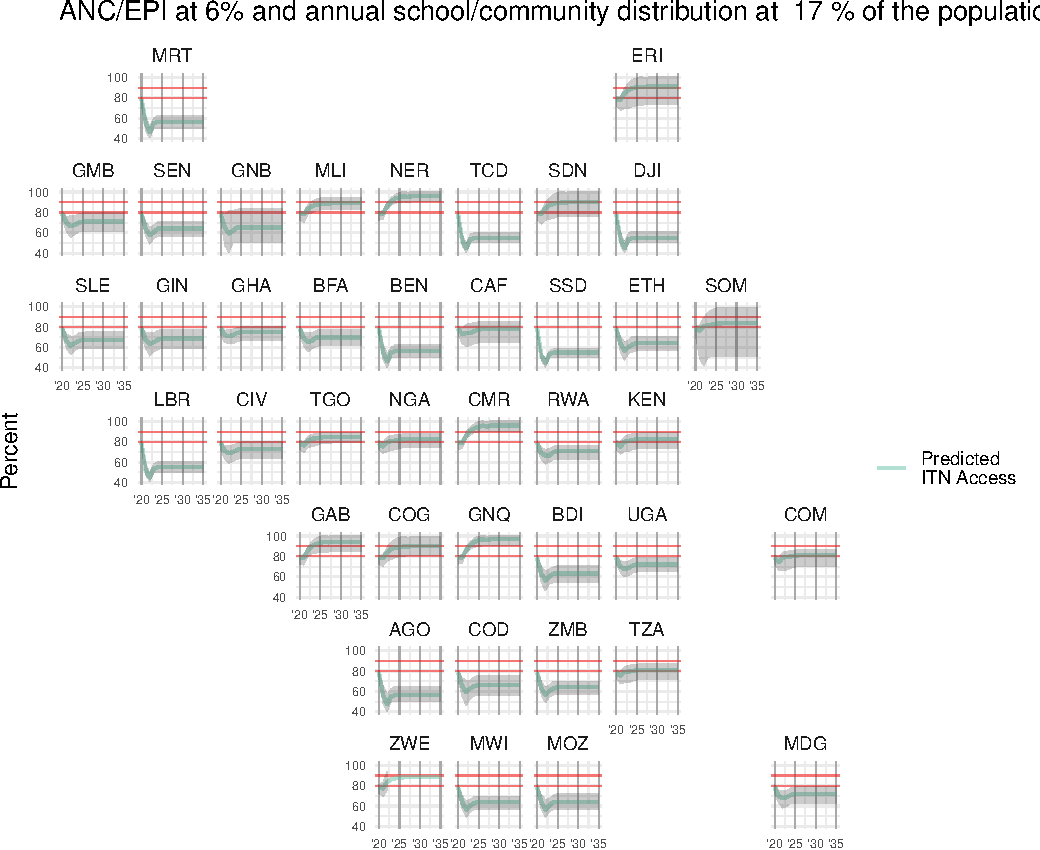
\includegraphics[width=0.8\linewidth]{quant_paper_files/figure-latex/geo_facets_cd-1}
\textbackslash caption\{\label{geo_facets_cd}Estimated ITN access with
annual ANC/EPI at 6\% and full continuous distribution strategy at 17\%
of the population in nets each year. Shaded areas indicate 95\%
confidence intervals accounting for both net retention times and ITN
access as a function of nets-per-capita (NPC)\}\label{fig:geo_facets_cd}
\textbackslash end\{figure\}

even more test stuff

\textbackslash begin\{figure\}
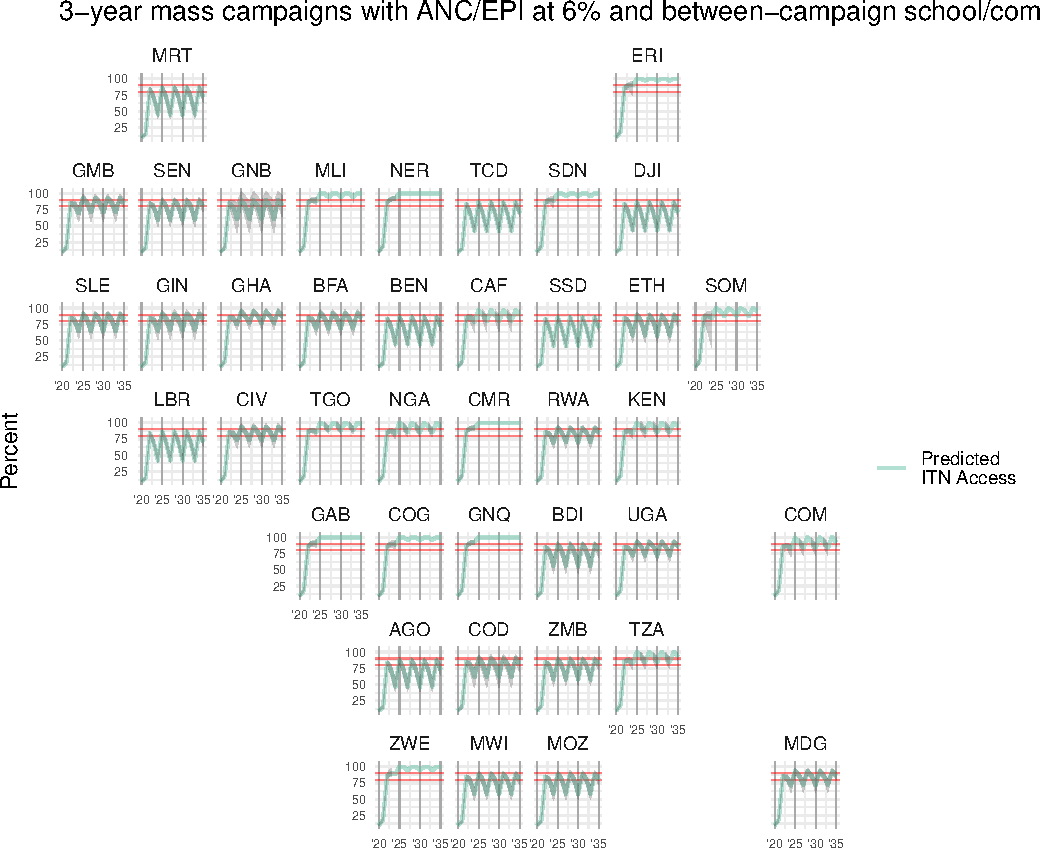
\includegraphics[width=0.8\linewidth]{quant_paper_files/figure-latex/geo_facets_cducc-1}
\textbackslash caption\{\label{geo_facets_cducc}Scenario 3 - three-year
mass campaigns with ANC/EPI distribution at 6\%, and between-campaign
continuous distribution at 10\%\}\label{fig:geo_facets_cducc}
\textbackslash end\{figure\}

The complete set of graphs for all scenarios is included as Supplemental
File 1.

Table 5 summarizes the recommended quantifiers under each scenario,
given a target of maintaining 80\% population ITN access.

\textbackslash begin\{table\}

\textbackslash caption\{\label{tab:kable_table80}Summary of recommended
quantifiers for scenarios, to maintain ITN access at or above 80\%\}
\centering

\begin{tabular}[t]{l|r|r|r|r}
\hline
\multicolumn{1}{c|}{ } & \multicolumn{2}{c|}{Continuous Distribution} & \multicolumn{2}{c}{Mass Campaign} \\
\cline{2-3} \cline{4-5}
Country & Full-scale continuous + routine & Campaign + routine + continuous between campaigns & 3-yearly campaigns & 2-yearly campaigns\\
\hline
Angola & 30 & 29 &  & 1.1\\
\hline
Burkina Faso & 25 & 17 &  & 1.7\\
\hline
Burundi & 29 & 23 &  & 1.4\\
\hline
Benin &  & 30 &  & 1.1\\
\hline
Congo - Kinshasa & 28 & 21 &  & 1.5\\
\hline
Central African Republic & 24 & 10 & 1.0 & \\
\hline
Congo - Brazzaville & 12 & 7 & 1.7 & \\
\hline
Côte d’Ivoire & 29 & 14 &  & 1.9\\
\hline
Cameroon & 10 & 7 & 2.0 & \\
\hline
Djibouti &  & 21 &  & 1.0\\
\hline
Eritrea & 12 & 7 & 1.8 & \\
\hline
Ethiopia & 29 & 23 &  & 1.4\\
\hline
Gabon & 10 & 7 & 2.0 & \\
\hline
Ghana & 27 & 7 &  & \\
\hline
Gambia & 25 & 16 &  & 1.8\\
\hline
Guinea & 26 & 19 &  & 1.6\\
\hline
Equatorial Guinea & 10 &  & 2.0 & \\
\hline
Guinea-Bissau & 28 & 22 &  & 1.4\\
\hline
Kenya & 17 & 7 & 1.3 & \\
\hline
Comoros & 19 & 8 & 1.2 & \\
\hline
Liberia &  & 22 &  & 1.0\\
\hline
Madagascar & 24 & 15 &  & 1.8\\
\hline
Mali & 12 & 7 & 1.7 & \\
\hline
Mauritania &  & 30 &  & 1.1\\
\hline
Malawi & 29 & 23 &  & 1.4\\
\hline
Mozambique & 28 & 23 &  & 1.4\\
\hline
Niger & 10 & 7 & 2.0 & \\
\hline
Nigeria & 18 & 7 & 1.3 & \\
\hline
Rwanda & 25 & 17 &  & 1.7\\
\hline
Sudan & 12 & 7 & 1.7 & 2.0\\
\hline
Sierra Leone & 27 & 20 &  & 1.6\\
\hline
Senegal & 28 & 22 &  & 1.4\\
\hline
Somalia & 16 & 7 & 1.4 & \\
\hline
South Sudan &  & 22 &  & 1.0\\
\hline
Chad &  & 22 &  & 1.0\\
\hline
Togo & 15 & 7 & 1.4 & \\
\hline
Tanzania & 19 & 8 & 1.2 & \\
\hline
Uganda & 24 & 15 &  & 1.8\\
\hline
Zambia & 29 & 23 &  & 1.4\\
\hline
Zimbabwe & 12 & 7 & 1.7 & \\
\hline
\end{tabular}

\textbackslash end\{table\}

Adjustments in quantification for ANC-EPI distribution did not lead to
large differences in ITN access in Scenario 1. The key factors driving
variation across countries within a given scenario were the estimated
retention times for each country.

Using the most recent Demographic and Health Survey, the proportion of
the population that were primary school students currently attending
school was calculated and compared to the population quantifiers needed
to achieve 70\% and 80\% ITN access targets in Scenario 2. Countries
where the proportion of primary school students attending school met or
exceeded the population quantifier are shown in Figure 5, as an
indication of where annual school distribution would be feasible. This
assumes that only one ITN is given per pupil; for the orange countries
in Figure 5, giving more than 1 ITN per pupil could provide a solution.

\hypertarget{discussion}{%
\section{Discussion}\label{discussion}}

\begin{itemize}
\tightlist
\item
  Mass campaigns + ANC-EPI (7\%) produces low access for most countries
\item
  Approach 80\% access when Cameroon at 15\%; TZA requires 22\%; Liberia
  at 25\% is still only 60\%
\item
  X\% of countries won't reach 80\% even at 25\%\ldots.
\item
  Ghana needs X and is only doing Y
\item
  What is the lowest access we are willing to tolerate between
  campaigns, or at any time\ldots?
\item
  2-year campaigns\ldots.?????
\item
  Link back to 4 questions from the Intro
\item
  No wonder no one is meeting 80\% targets
\item
  If we want 80\% ITN use we would need 90\% access as the target
\item
  Based on projections across multiple countries using varying ITN
  retention times from Bertozzi-Villa, overall recommendations for CD
  and campaign quantification for other countries
\item
  Providing greater and greater numbers of nets/more frequently
  disincentivizes retention times (?)
\item
  Limitation of the methods

  \begin{itemize}
  \tightlist
  \item
    Parameter assumptions - decay rates, some countries with limited
    data; rates expected to vary within the country; (behaviors; nets)
  \item
    Relationship between Nets-as-proportion-of-population and ITN access
    may be different under a Scenario 1 vs a Scenario 2, depending on
    the degree of oversaturation inherent in the distribution channel
    (schools; etc).
  \end{itemize}
\end{itemize}

\hypertarget{conclusion}{%
\section{Conclusion}\label{conclusion}}

Given variation in ITN retention times across countries, tailored
quantification approaches for mass campaigns and continuous distribution
strategies are warranted. To reach target levels of ITN use of 80\% of
the population, ITN access must be maintained near 90\% in most
settings. The quantity of ITNs required to meet these goals are
substantially larger than current plans. National programmes and their
funding partners should work to increase the number of ITNs distributed
to those vulnerable to malaria, while at the same time working to extend
the useful life of these critical commodities.

\hypertarget{declarations}{%
\section{Declarations}\label{declarations}}

\hypertarget{ethics-approval-and-consent-to-participate}{%
\subsection{Ethics approval and consent to
participate}\label{ethics-approval-and-consent-to-participate}}

Not applicable

\hypertarget{consent-for-publication}{%
\subsection{Consent for publication}\label{consent-for-publication}}

Not applicable

\hypertarget{availability-of-data-and-materials}{%
\subsection{Availability of data and
materials}\label{availability-of-data-and-materials}}

Code is available at https://github.com/hkoenker/

\hypertarget{competing-interests}{%
\subsection{Competing interests}\label{competing-interests}}

The authors declare that they have no competing interests.

\hypertarget{funding}{%
\subsection{Funding}\label{funding}}

HK was supported through a grant from The Bill \& Melinda Gates
Foundation.

\hypertarget{authors-contributions}{%
\subsection{Authors' contributions}\label{authors-contributions}}

\hypertarget{acknowledgements}{%
\subsection{Acknowledgements}\label{acknowledgements}}

\hypertarget{authors-information-optional}{%
\subsection{Authors' information
(optional)}\label{authors-information-optional}}

\hypertarget{supplementary-information}{%
\section{Supplementary information}\label{supplementary-information}}

\renewcommand\refname{References}
\bibliography{quantbibfile.bib}


\end{document}
